\documentclass[a4paper,twoside,12pt]{report}
% Richard Klein (2020,2021)

% Include Packages
%\usepackage[a4paper,inner=3.5cm,outer=2.5cm,top=2.5cm,bottom=2.5cm]{geometry}  % Set page margins
\usepackage{fullpage}
\usepackage{float}                  % Allows 'Here and Only Here' [H] for Floats
\usepackage{url}                    % \url{} command
\usepackage{charter}                  % Set font to Times
\usepackage{graphicx}               % \includegraphics
\usepackage{subfigure}              % Allow subfigures
\usepackage{amsmath}
\usepackage{amssymb}
\usepackage{amsthm}
\usepackage{booktabs}
\usepackage{parskip}
\usepackage{pgfgantt}
\usepackage[dvipsnames]{xcolor}
\usepackage[all]{nowidow}
\setnoclub[2]
\setnowidow[2]

% Referencing
% Provides \Vref and \vref to indicate where a reference is.
\usepackage{varioref} 
% Hyperlinks references
\usepackage[bookmarks=true,bookmarksopen=true]{hyperref} 
% Provides \Cref, \cref, \Vref, \vref to include the type of reference: fig/eqn/tbl
\usepackage{cleveref} 
% Setup Hyperref
\hypersetup{
  colorlinks   = true,              %Colours links instead of ugly boxes
  urlcolor     = blue,              %Colour for external hyperlinks
  linkcolor    = blue,              %Colour of internal links
  citecolor    = blue                %Colour of citations
}
% Names for Clever Ref
\crefname{table}{table}{tables}
\Crefname{table}{Table}{Tables}
\crefname{figure}{figure}{figures}
\Crefname{figure}{Figure}{Figures}
\crefname{equation}{equation}{equations}
\Crefname{equation}{Equation}{Equations}

% Wits Citation Style
\usepackage{natbib} \input{natbib-add}
\bibliographystyle{named-wits}
\bibpunct{[}{]}{;}{a}{}{}  % to get correct punctuation for bibliography
\setlength{\skip\footins}{1.5cm}
\newcommand{\citets}[1]{\citeauthor{#1}'s \citeyearpar{#1}}
\renewcommand\bibname{References}  

\pagestyle{headings}

\pagestyle{plain}
\pagenumbering{roman}

\renewenvironment{abstract}{\ \vfill\begin{center}\textbf{Abstract}\end{center}\addcontentsline{toc}{section}{Abstract}}{\vfill\vfill\newpage}
\newenvironment{declaration}{\ \vfill\begin{center}\textbf{Declaration}\end{center}\addcontentsline{toc}{section}{Declaration}}{\vfill\vfill\newpage}
\newenvironment{aideclaration}{\ \vfill\begin{center}\textbf{AI Declaration}\end{center}\addcontentsline{toc}{section}{AI Declaration}}{\vfill\vfill\newpage}
\newenvironment{acknowledgements}{\ \vfill\begin{center}\textbf{Acknowledgements}\end{center}\addcontentsline{toc}{section}{Acknowledgements}}{\vfill\vfill\newpage}

\begin{document}
\onecolumn
\thispagestyle{empty}

\setcounter{page}{0}
\addcontentsline{toc}{chapter}{Preface}
\ 
\begin{center}
  \vfill
  {
  \huge \bf \textsc{Diffusion-Based Refinement of Textual Conditioning for Improved Generative Modeling}\\
  \large Enhancing Compositional Fidelity via Semantic Refinement of Textual Conditioning
  \\[20pt]
  \large School of Computer Science \& Applied Mathematics\\
  \large University of the Witwatersrand\\[20pt]
  \normalsize
Oratile Nailana\\
  2327853\\[20pt]
  Supervised by Dr. Devon Jarvis\\[10pt]
  \today
  }

  \vfill
  \vfill
  
\includegraphics[width=1.5cm]{images/wits}
  \vspace{10pt}\\
  \small{A proposal submitted to the Faculty of Science, University of the Witwatersrand, Johannesburg,
in partial fulfilment of the requirements for the degree of Master of Science}\\
\end{center}
\vfill
\newpage

\pagestyle{plain}
\setcounter{page}{1}

\phantomsection
\begin{abstract}
Recent advances in text-to-image (T2I) diffusion models have demonstrated strong generative capabilities, yet their performance remains fundamentally dependent on the quality of textual conditioning. In practice, prompts are often too short and ambiguous to fully specify complex scenes and object relationships. This frequently results in compositional errors and object entanglement, while also making generation highly sensitive to the choice of guidance parameters. While prior work has largely focused on scaling model architectures and introducing auxiliary control signals, the semantic quality of textual conditioning has received comparatively limited attention. Natural language prompts provide only a compressed and discrete representation of a user’s intended scene, often omitting contextual, relational and attribute-level information that remains implicit in human communication. Consequently, we interpret textual prompts as noisy observations of an underlying semantic signal and propose diffusion as a principled mechanism for estimating and refining this signal prior to conditioning.

We investigate whether diffusion-based refinement of textual inputs produces more informative conditioning signals for T2I diffusion. Rather than modifying the image generation backbone, the proposed approach uses GENIE to expand user prompts into semantically enriched representations that explicitly describe objects, their attributes, spatial relationships and scene composition. The refined prompts are then used directly by the T2I model without requiring any changes to the existing generation system, while still providing clearer and more informative guidance for image generation.

The central hypothesis is that stronger compositional structure in the conditioning signal translates into improved compositional generation in image space. Natural language explicitly represents role–filler associations between objects, attributes and spatial relations, whereas these bindings become increasingly distributed and difficult to preserve during visual diffusion. We therefore investigate whether refined prompts provide stronger semantic constraints for downstream generation, improving attribute binding and relational correctness while reducing sensitivity to classifier-free guidance.

The expected contribution of this work is a clearer understanding of conditioning quality as a bottleneck in diffusion based image generation and empirical evidence for whether refining textual conditioning via diffusion can improve controllability, robustness and compositional generation without requiring changes to the underlying diffusion model architecture.
\end{abstract}

\phantomsection
\begin{declaration}
I, Oratile Nailana, hereby declare the contents of this research proposal to be my own work.
This proposal is submitted for the degree of Master of Science in Computer Science at the University of the Witwatersrand.
This work has not been submitted to any other university, or for any other degree.
\end{declaration}




\phantomsection
\addcontentsline{toc}{section}{Table of Contents}
\tableofcontents
\newpage
\phantomsection
% \addcontentsline{toc}{section}{List of Figures}
\newpage
\newpage
\pagenumbering{arabic}

\chapter{Introduction}
Recent advances in image generation have been driven by deep generative models. Early GAN-based approaches demonstrated high-fidelity image synthesis but were often hindered by training instability and mode collapse, limiting robustness and diversity of outputs \citep{goodfellow2014generative, salimans2016improved, arjovsky2017wasserstein}. Subsequent probabilistic approaches such as variational autoencoders and autoregressive models improved
theoretical grounding but struggled to scale effectively to high-resolution image synthesis\citep{kingma2013auto, rezende2014stochastic}. 


More recently, diffusion probabilistic models have emerged as a leading paradigm. Formalised through denoising diffusion probabilistic models (DDPMs), they learn to reverse a gradual noising process enabling stable training and
high quality sample generation \citep{ho2020ddpm, song2021score}. These models were further scaled and made computationally efficient through latent diffusion, where generation is performed in a compressed latent space rather than pixel space \citep{rombach2022ldm}. This formulation underpins modern large-scale text-to-image systems such as Stable Diffusion \citep{rombach2022ldm}, which combines latent diffusion with powerful text encoders to enable high-quality conditional image synthesis.

A key enabling component of these systems is CLIP \citep{radford2021clip}, which learns a shared embedding space between text and images via contrastive learning. In diffusion pipelines, CLIP encoders map discrete textual prompts into continuous semantic representations that condition the denoising process. However, this introduces a fixed semantic bottleneck, where downstream generation becomes constrained by the expressiveness and compositional fidelity of the text embedding produced by the encoder.

Despite strong generative performance, T2I diffusion models remain sensitive to prompt formulation. Natural language prompts are often underspecified and lack explicit compositional structure describing objects, attributes and their relationships. This leads to persistent failures in compositional generation, particularly in attribute binding and relational consistency, as demonstrated in studies such as Composable Diffusion Models \citep{liu2022composable} and recent benchmark evaluations \citep{huang2023t2icompbench}.

From a signal processing perspective, textual conditioning in T2I diffusion models can be interpreted as a noisy observation of an underlying semantic intent. In this view, a user prompt encodes both structured semantic content and residual ambiguity arising from the discrete and compressed nature of natural language. Furthermore, studies on ambiguity in T2I generation demonstrate that existing diffusion models often struggle to resolve underspecified prompts and recover fine-grained relational and attribute-level information from textual descriptions alone \citep{huang2023t2icompbench, mehrabi2023ambiguities, elsharif2025ambiguity}. As a result, the encoded conditioning signal may be viewed as an incomplete representation of the underlying semantic structure required for accurate image synthesis.

To mitigate these issues, classifier-free guidance (CFG) has become a standard mechanism for improving prompt-image alignment in diffusion models \citep{ho2022cfg}. CFG improves prompt adherence by amplifying conditional information during generation, but introduces strong sensitivity to guidance scale and often requires careful tuning to balance fidelity and diversity.

In parallel, attention-based control methods provide insight into how textual information is grounded in image generation.  \cite{hertz2022prompt} demonstrate that manipulating cross-attention maps enables fine-grained editing of generated images without retraining the model. However, these methods remain dependent on the initial quality of the text embedding produced by fixed encoders such as CLIP.

More recently, structural conditioning approaches such as ControlNet and T2I-Adapter introduce auxiliary control signals, including edges, depth maps, and segmentation masks, to improve spatial fidelity and controllability \citep{zhang2023controlnet, mou2023t2iadapter}.

Diffusion language models extend the diffusion paradigm to discrete token spaces, enabling iterative refinement of text through a denoising process \citep{ li2022diffusionlm}. Unlike autoregressive models, these approaches treat language generation as progressive structure recovery from noise, offering a principled mechanism for semantic refinement. This suggests that discrete token sequences may be interpreted as partially corrupted observations from which latent structure can be iteratively recovered through denoising \citep{austin2021structured}.

To the best of our knowledge, limited work has investigated whether diffusion-based refinement in language space can improve the conditioning quality of downstream T2I diffusion models. Existing approaches primarily focus on modifying image generation architectures or incorporating auxiliary conditioning signals to improve spatial control and fidelity \citep{hertz2022prompt, zhang2023controlnet, mou2023t2iadapter, saharia2022imagen}. In contrast, comparatively little attention has been given to improving the semantic structure of the textual conditioning signal itself prior to image synthesis.

This raises the question of whether iterative semantic refinement and expansion of prompts into richer textual descriptions can produce more stable and compositionally informative conditioning representations for downstream diffusion models. From this perspective, textual prompts may be interpreted as compressed observations of a richer latent semantic structure that is only partially expressed through discrete language tokens \citep{li2022diffusionlm, austin2021structured}.
\section*{Structure of the Proposal}

This research proposal investigates whether diffusion-based semantic refinement of textual prompts can improve compositional consistency and conditioning quality in text-to-image diffusion models. The proposed study explores the use of diffusion language models to iteratively expand and refine prompts before they are processed by the underlying text-to-image system, with the goal of reducing ambiguity and improving attribute binding, object relationships, and overall semantic alignment in generated images.

The proposal is organised as follows. Chapter 2 reviews the theoretical foundations and related work underlying generative modelling and text-conditioned diffusion systems. Chapter 3 presents the research questions, hypotheses, and proposed methodology guiding the study, including the experimental setup and evaluation framework. Chapter 4 outlines the proposed research plan, practical considerations, and anticipated limitations of the study. Finally, Chapter 5 concludes the proposal by summarising the intended contributions and discussing potential directions for future research.

\begin{itemize}
    \item \textbf{Chapter 2: Background and Related Work}  
    Reviews generative modelling, diffusion models, text conditioning, and prior work related to compositional text-to-image generation.

    \item \textbf{Chapter 3: Research Questions, Hypotheses and Methodology}  
    Defines the research questions and hypotheses, and describes the proposed prompt refinement framework, experimental design, datasets, and evaluation metrics.

    \item \textbf{Chapter 4: Research Plan}  
    Presents the proposed implementation strategy, timeline, computational requirements, and anticipated challenges.

    \item \textbf{Chapter 5: Conclusion}  
    Summarises the proposed research objectives, expected contributions, and future research directions.
\end{itemize}

This structure is intended to build a logical progression from problem formulation to proposed implementation, ensuring the research is grounded in theory while remaining focused on practical experimentation and evaluation.




\chapter{Background and Related Work}

% =========================================================

\section{Generative Modelling}

\textbf{Generative modelling} involves learning the probability distribution underlying a training dataset, allowing a model to generate new samples that resemble the original data \citep{goodfellow2016deep, bishop2006pattern}. Discriminative models focus on learning the conditional distribution $p(y \mid x)$, directly modelling the relationship between inputs and outputs for prediction. In contrast, generative models aim to capture the underlying data distribution, typically by modelling $p(x)$ or the joint distribution $p(x, y)$  \citep{murphy2022probabilistic}. Given observations \(x\), a generative model seeks to approximate the probability distribution \(p(x)\), enabling sampling and learning of complex high-dimensional data distributions \citep{bishop2006pattern, kingma2019introduction}.

Many generative modelling approaches are grounded in probabilistic reasoning and Bayesian inference \citep{mackay2003information}. In Bayesian inference, we usually want to compute a posterior distribution over the parameters \(\theta\) given the observed data \(x\). From Bayes’ theorem:

\begin{equation}
    p(\theta \mid x) = \frac{p(x \mid \theta)p(\theta)}{p(x)}
\end{equation}

where:
\begin{itemize}
    \item \(p(\theta)\) = prior distribution
    \item \(p(x \mid \theta)\) = likelihood
    \item \(p(x)\) = marginal likelihood/evidence
    \item \(p(\theta \mid x)\) = posterior distribution
\end{itemize}

The evidence term \(p(x)\) is defined as:
\begin{equation}
    p(x) = \int p(x \mid \theta)p(\theta)\,d\theta
\end{equation}

For modern high-dimensional models, exact inference is intractable, motivating approximate inference and scalable deep learning approaches \citep{blei2017variational, murphy2022probabilistic}.

% =========================================================

\subsection{Approximate Inference and Learning in High Dimensions}

With exact Bayesian inference being generally intractable in modern generative models, approximate inference methods are required to enable learning and sampling in high-dimensional parameter spaces \citep{mackay2003information, bishop2006pattern, murphy2022probabilistic}.

Variational inference introduces a tractable surrogate distribution \(q(\theta)\) to approximate the true posterior \(p(\theta \mid x)\). The quality of this approximation is optimised by maximising the Evidence Lower Bound (ELBO), which provides a lower bound on the marginal likelihood \citep{blei2017variational, kingma2013auto}:

\begin{equation}
\log p(x) \geq \mathbb{E}_{q(\theta)}[\log p(x \mid \theta)] - KL(q(\theta)\|p(\theta))
\end{equation}

This formulation reframes inference as an optimisation problem, where learning proceeds by minimising the divergence between an approximate and true posterior distribution. However, the choice of variational family \(q(\theta)\) introduces a trade-off between tractability and expressiveness, often limiting the quality of posterior approximations in complex models \citep{blei2017variational}.

An alternative approach is provided by Monte Carlo methods, particularly Markov Chain Monte Carlo (MCMC), which construct samples from the posterior distribution via stochastic simulation. While asymptotically exact, these methods are computationally expensive and difficult to scale to modern deep learning architectures with millions or billions of parameters \citep{neal2011mcmc, robert2004montecarlo}.

To address these limitations, amortised inference has been introduced in latent variable models such as variational autoencoders. Instead of optimising a separate variational distribution for each data point, amortised inference learns a parameterised mapping from data to latent representations. This significantly improves scalability and enables efficient inference at test time, but introduces an amortisation gap arising from restricting inference to a shared parameterised function class rather than optimising a per-datapoint variational distribution \citep{kingma2013auto, rezende2014stochastic, margossianblei2023amortized}.

% =========================================================



\subsection{Deep Generative Models}

Deep generative models can be understood as scalable parameterisations of probabilistic models that learn complex data distributions using neural networks. They learn parameterised probability distributions over data via optimisation-based objectives, rather than relying on closed-form inference.

Within this paradigm, three foundational classes of deep generative models are commonly studied: variational autoencoders, generative adversarial networks, and autoregressive models. Each class reflects a different compromise between likelihood-based modeling, sample generation efficiency and, inference and learning structure.

\subsection{Variational Autoencoders}

Variational autoencoders (VAEs) can be interpreted as a principled instantiation of amortised variational inference in deep latent variable models \citep{kingma2013auto, rezende2014stochastic, margossianblei2023amortized}. They introduce latent variables \(z\) and define a generative process of the form:

\begin{equation}
p_\theta(x, z) = p_\theta(x \mid z)p(z)
\end{equation}

where \(p(z)\) is typically chosen as a simple prior such as a standard Gaussian distribution.

Since the true posterior \(p(z \mid x)\) is intractable, VAEs introduce a learned approximate posterior \(q_\phi(z \mid x)\), parameterised by an encoder neural network. This formulation directly corresponds to amortised inference, where inference is shared across all datapoints through a single parameterised function \citep{margossianblei2023amortized}.

Training is performed by maximising the Evidence Lower Bound (ELBO):

\begin{equation}
\mathcal{L}_{ELBO} = \mathbb{E}_{q_\phi(z|x)}[\log p_\theta(x|z)] - KL(q_\phi(z|x)\|p(z))
\end{equation}

The first term encourages accurate reconstruction of the data, while the second regularises the latent space to remain close to the prior distribution, ensuring a well-behaved latent structure that supports efficient sampling and prevents arbitrary divergence of encoded representations.

This optimisation procedure may be interpreted as jointly learning a latent representation space and an approximate inference mechanism. However, the reliance on a simple prior distribution and the Gaussian assumption in the approximate posterior impose strong structural constraints on the learned representation space \citep{kingma2013auto}.

As a result, VAEs often produce samples that are smooth and coherent but lack sharpness and fine-grained detail. This is commonly attributed to the variational objective encouraging conservative approximations of the data distribution, as well as limitations in the expressiveness of the amortised inference network \citep{bowman2016generating, kingma2019introduction}.

More fundamentally, VAEs illustrate a key trade-off in deep generative modelling: scalability through amortised inference comes at the cost of posterior approximation bias and restricted representational flexibility.

\subsection{Generative Adversarial Networks}

Generative adversarial networks (GANs) formulate generative modelling as a minimax game between a generator \(G\) and a discriminator \(D\) \citep{goodfellow2014generative}. The generator learns to map samples from a latent prior \(z \sim p(z)\) to data space, while the discriminator attempts to distinguish real data from generated samples. This adversarial objective is defined as:

\begin{equation}
\min_G \max_D \mathbb{E}_{x \sim p_{data}}[\log D(x)] + \mathbb{E}_{z \sim p(z)}[\log(1 - D(G(z)))]
\end{equation}

Unlike likelihood-based models such as VAEs, GANs do not explicitly define or optimise a tractable probability density. Instead, they implicitly learn to match the data distribution through adversarial feedback.

GANs are capable of producing high-fidelity and sharp samples, particularly in image generation tasks. However, training is notoriously unstable due to the adversarial optimisation dynamics, which can lead to non-convergence and sensitivity to hyperparameter selection. Additionally, GANs are prone to mode collapse, where the generator learns to produce only a subset of the data distribution, reducing diversity in generated samples \citep{salimans2016improved, arjovsky2017wasserstein}.

While GANs were historically significant in advancing high-quality image synthesis, they have largely been superseded in large-scale conditional generation tasks by diffusion-based models, which offer more stable training dynamics and better coverage of the data distribution.

\subsection{Autoregressive Models}

Autoregressive models define a probability distribution over high-dimensional data by factorising the joint distribution into a product of conditional distributions:

\begin{equation}
p(x) = \prod_{i=1}^{n} p(x_i \mid x_{<i})
\end{equation}

This factorisation allows the model to be trained using exact maximum likelihood estimation, since each conditional distribution is explicitly modelled. Autoregressive architectures such as PixelRNN, PixelCNN, and Transformer-based language models have demonstrated strong performance across both image and sequence modelling tasks \citep{van2016pixelrnn, oord2016pixelcnn, vaswani2017attention}.

However, a key limitation of autoregressive modelling lies in its inherently sequential generation process. Sampling requires iterative evaluation of each conditional distribution, making generation computationally expensive and poorly parallelisable. This results in slow inference times, particularly for high-dimensional data such as images, where the number of required generation steps scales with the number of pixels or tokens. The strictly sequential factorisation of autoregressive models prevents global refinement of earlier decisions, as each token is generated conditioned on previously fixed outputs.

Despite this limitation, autoregressive models remain a fundamental baseline in generative modelling due to their exact likelihood formulation and strong theoretical grounding in probabilistic sequence modelling.

% =========================================================

\section{Diffusion Probabilistic Models}

Diffusion models define a generative process as the reversal of a gradual noising procedure\citep{ho2020ddpm,song2021score}. A forward process progressively corrupts data with Gaussian noise according to a Markov chain formulation:

The forward diffusion process is defined as a fixed Markov chain that gradually injects Gaussian noise into the data distribution:

\begin{equation}
q(x_t|x_{t-1}) = \mathcal{N}(x_t; \sqrt{1 - \beta_t}x_{t-1}, \beta_t I)
\end{equation}

where:
\begin{itemize}
    \item \(x_{t-1}\) is the data sample at timestep \(t-1\),
    \item \(x_t\) is the noised sample at timestep \(t\),
    \item \(\beta_t \in (0,1)\) is a predefined variance schedule controlling the amount of noise injected at each step,
    \item \(I\) denotes the identity covariance matrix, implying isotropic Gaussian noise.
\end{itemize}

This Markovian construction ensures that noise is incrementally accumulated over time, leading to a progressively corrupted version of the original data distribution \citep{ho2020ddpm}.


\begin{figure}[ht]
    \centering
    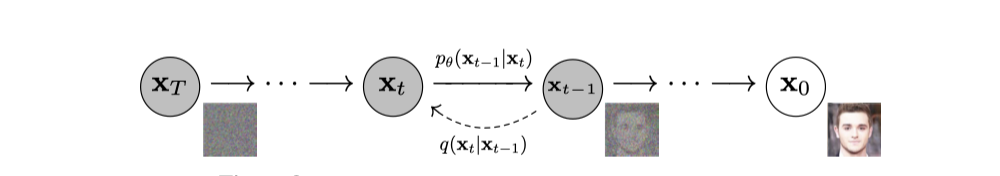
\includegraphics[width=1\textwidth]{images/DDPM-markovian-chain.png}
    \caption{Illustration of markovian chain in the context of DDPM. Adapted from \citet{ho2020ddpm}.}
\end{figure}

The closed-form marginal distribution at timestep \(t\) can be expressed as:

\begin{equation}
x_t = \sqrt{\bar{\alpha}_t}x_0 + \sqrt{1 - \bar{\alpha}_t}\epsilon, \quad \epsilon \sim \mathcal{N}(0, I)
\end{equation}

where:
\begin{itemize}
    \item \(x_0\) denotes the original data sample,
    \item \(x_t\) is the noisy version of the data at diffusion timestep \(t\),
    \item \(\epsilon\) is standard Gaussian noise,
    \item \(\alpha_t = 1 - \beta_t\),
    \item \(\bar{\alpha}_t = \prod_{s=1}^{t} \alpha_s\) is the cumulative product of noise scheduling coefficients.
\end{itemize}

This reparameterisation is central to efficient training, as it allows direct sampling of noisy data points without simulating the full Markov chain \citep{ho2020ddpm, nichol2021improved}.

The reverse generative process is learned by training a neural network to predict the noise component:

\begin{equation}
\epsilon_\theta(x_t, t)
\end{equation}

with the standard simplified training objective:

\begin{equation}
\mathcal{L} = \mathbb{E}_{x_0, \epsilon, t}\left[||\epsilon - \epsilon_\theta(x_t, t)||^2\right]
\end{equation}

This objective can be interpreted as learning a denoising direction at each noise level, effectively learning a sequence of progressively refined estimates of the data distribution across noise scales \citep{ho2020ddpm, song2021scorebasedgenerative}.

From a probabilistic perspective, this corresponds to learning the score of the data distribution under progressive corruption, linking diffusion models to score matching formulations \citep{hyvarinen2005score,song2021score}.

Denoising Diffusion Implicit Models (DDIMs) extend this framework by introducing a non-Markovian deterministic sampling process, enabling faster inference while preserving sample quality by constructing an implicit trajectory through the same learned score field \citep{song2022ddim}.

More recent work has also explored accelerating diffusion sampling through distillation and consistency training, reducing the number of required denoising steps while preserving fidelity \citep{salimans2022progressivedistillation,song2023consistency}.
% =========================================================
\subsection{Score-Based Generative Modelling}

Score-based generative models provide a continuous-time formulation of diffusion by directly estimating the score function:

\begin{equation}
\nabla_x \log p(x)
\end{equation}

This quantity represents the gradient of the log-density and provides a direction of increasing probability under the data distribution \citep{hyvarinen2005score}. A neural network \(s_\theta(x_t, t)\) is trained to approximate this score using denoising score matching objectives \citep{vincent2011connection,song2021score}.

The forward process is defined via a stochastic differential equation (SDE):

\begin{equation}
dx_t = f(x_t, t)\,dt + g(t)\,dW_t
\end{equation}

where different choices of drift and diffusion functions give rise to variance-preserving (VP), variance-exploding (VE), and sub-VP formulations \citep{song2021scorebasedgenerative}.

Sampling is performed using the reverse-time SDE:

\begin{equation}
dx_t = \left[f(x_t, t) - g(t)^2 \nabla_x \log p_t(x_t)\right]dt + g(t)\,d\bar{W_t}
\end{equation}

This formulation establishes diffusion models as solutions to a time-reversal problem over stochastic processes, where generation corresponds to integrating a learned vector field backward in time \citep{anderson1982reverse, song2021scorebasedgenerative}.

This continuous-time view unifies diffusion models with probability flow ordinary differential equations (ODEs), enabling deterministic sampling through numerical integration of the learned score field \citep{song2021scorebasedgenerative}.

\begin{figure}[ht]
    \centering
    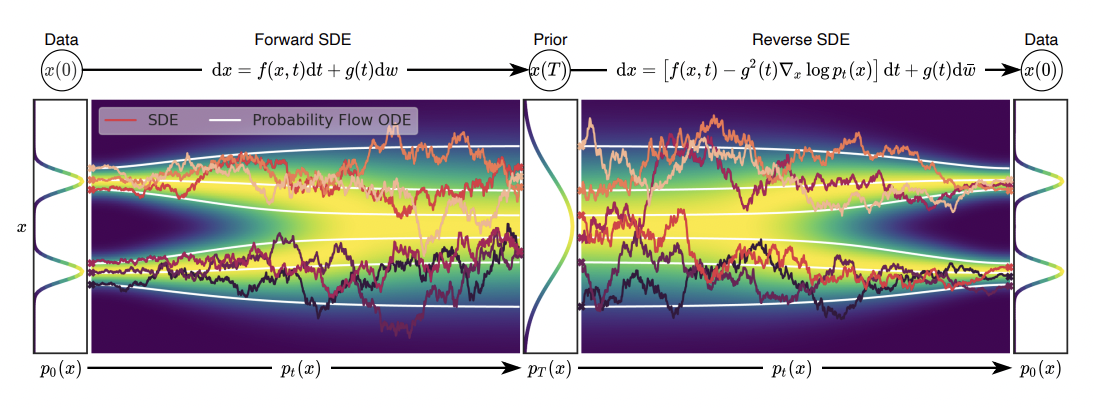
\includegraphics[width=0.9\textwidth]{images/overview-score-based.png}
    \caption{Score-based generative modelling via stochastic differential equations. Adapted from \citet{song2021score}.}
\end{figure}
\subsubsection{Product-of-Experts Conditioning}

Product-of-Experts (PoE) provides a compositional probabilistic framework in which multiple conditional distributions are combined multiplicatively to form a joint distribution \citep{hinton2002training, du2019implicit, liu2022compositional}:

\begin{equation}
p(x)
=
\frac{1}{Z}
\prod_{i=1}^{N}
p_i(x)
\end{equation}

Taking the logarithm and differentiating yields:

\begin{equation}
\nabla_x \log p(x)
=
\sum_{i=1}^{N}
\nabla_x \log p_i(x)
\end{equation}

Thus, under a Product-of-Experts formulation, individual score functions contribute additively to the overall denoising direction.

Within diffusion-based generation, this enables compositional conditioning by treating prompt components such as objects, attributes, or relations as separate conditional experts whose scores are combined during sampling \citep{liu2022compositional, du2020improved}.

Although Product-of-Experts conditioning is not directly used in the proposed methodology, it provides important theoretical context for compositional diffusion modelling. In particular, it illustrates how multiple semantic constraints may be combined within score-based generation frameworks, while also highlighting challenges such as expert conflict, unstable guidance trajectories, and semantic entanglement under imperfect conditioning.
% =========================================================
\subsection{Latent Diffusion Models}

To improve computational efficiency, diffusion models are often applied in a learned latent space rather than pixel space. This idea is closely related to latent variable modelling frameworks such as VAEs, which learn compressed representations of data through an encoder–decoder architecture and probabilistic latent space formulation.

In contrast to VAEs, where latent variables are sampled from a learned approximate posterior \(q_\phi(z|x)\), latent diffusion models replace explicit probabilistic inference with a deterministic encoding step, using a pretrained encoder to map data into a compact latent representation:

\begin{equation}
z = E(x)
\end{equation}

Diffusion is then performed in this latent space, and a decoder reconstructs the output:

\begin{equation}
x = D(z)
\end{equation}

This formulation significantly reduces computational cost while preserving the expressive power of diffusion models in high-dimensional data domains \citep{rombach2022ldm}.

Latent diffusion can therefore be interpreted as decoupling representation learning from generative modelling: the encoder–decoder pair provides a structured latent space, while the diffusion process models the distribution over that space.

This separation enables scalable high-resolution synthesis and forms the backbone of modern large-scale generative systems such as Stable Diffusion, where text-conditioning is injected into the latent denoising process via cross-attention mechanisms \citep{rombach2022ldm}.

% =========================================================
\subsection{Text-to-Image Diffusion Models}

Text-to-image diffusion models condition generation on textual inputs using pretrained language-image encoders such as CLIP \citep{radford2021clip}. These models learn a shared embedding space between text and images using a contrastive objective, aligning semantically related image-text pairs while separating unrelated ones \citep{radford2021clip, liu2022composable, saharia2022imagen}.

\subsubsection{CLIP-Based Text Conditioning}

CLIP encodes discrete text prompts into continuous semantic embeddings:

\begin{equation}
c = f_{\text{CLIP}}(t)
\end{equation}

where \(t\) denotes the input text prompt and \(c\) is the resulting conditioning vector. This embedding captures high-level semantic information and serves as the primary conditioning signal for downstream diffusion models \citep{radford2021clip, rombach2022ldm, saharia2022imagen}.

However, this formulation introduces a fixed semantic bottleneck: once the text is mapped into the embedding space, fine-grained compositional structure such as object relationships, spatial constraints, and attribute bindings may not be fully preserved. This limitation becomes particularly pronounced in complex prompts requiring multi-object reasoning or relational consistency \citep{liu2022composable, huang2023t2icompbench, mehrabi2023ambiguities, elsharif2025ambiguity}.

To inject conditioning into the generative process, modern diffusion models use cross-attention mechanisms within the U-Net architecture \citep{vaswani2017attention, rombach2022ldm}. At each denoising step, the image features attend to the textual embeddings:

\begin{equation}
\text{Attention}(Q, K, V) = \text{softmax}\left(\frac{QK^T}{\sqrt{d}}\right)V
\end{equation}

where queries \(Q\) originate from image features and keys/values \((K, V)\) are derived from the text conditioning vector \(c\). This mechanism enables spatial and semantic alignment between textual concepts and image regions \citep{vaswani2017attention, hertz2022prompt, rombach2022ldm}.

Cross-attention has also been shown to provide an interpretable interface for controlling generation, enabling localised edits and prompt manipulation without retraining the model \citep{hertz2022prompt}.
\subsubsection{Classifier-Free Guidance (CFG)}

Classifier-free guidance (CFG) is a widely used technique for improving prompt adherence in diffusion models by interpolating between conditional and unconditional noise predictions \citep{ho2022cfg, nichol2021improved}:

\begin{equation}
\hat{\epsilon}
=
(1 + w)\epsilon_\theta(x_t, c)
-
w\epsilon_\theta(x_t, \emptyset)
\end{equation}

where:
\begin{itemize}
    \item \(x_t\): noisy latent at timestep \(t\),
    \item \(c\): text conditioning embedding,
    \item \(\emptyset\): null conditioning,
    \item \(w\): guidance scale controlling conditioning strength.
\end{itemize}

CFG can be interpreted as steering sampling in the direction of the conditional score relative to the unconditional baseline, thereby amplifying the influence of the conditioning signal during generation \citep{ho2022cfg, song2021scorebasedgenerative, nichol2021improved}.

Rewriting the guidance formulation makes this interpretation explicit:

\begin{equation}
\hat{\epsilon}
=
\epsilon_\theta(x_t,\emptyset)
+
w\big(
\epsilon_\theta(x_t,c)
-
\epsilon_\theta(x_t,\emptyset)
\big)
\label{eq:cfg_decomposition}
\end{equation}

The second term represents the directional influence introduced by conditioning. As the guidance scale \(w\) increases, the denoising trajectory becomes increasingly dependent on the difference between conditional and unconditional predictions.

While CFG substantially improves prompt adherence, prior work has shown that it also introduces sensitivity to the guidance scale. Excessively large values of \(w\) can lead to oversaturation, artifact formation, reduced diversity, and unstable compositional behaviour \citep{ho2022cfg, saharia2022imagen, rombach2022ldm}.

These observations suggest that generation quality depends not only on the diffusion model itself, but also on the structure and reliability of the conditioning representation used during sampling. Recent studies further demonstrate that prompt ambiguity, incomplete semantic specification, and weak relational structure contribute significantly to compositional failures in text-to-image generation, particularly in multi-object and attribute-binding scenarios \citep{liu2022composable, huang2023t2icompbench, mehrabi2023ambiguities, elsharif2025ambiguity}.

Consequently, conditioning quality emerges as an important factor in determining how effectively semantic information is preserved and amplified throughout the denoising process. This motivates further investigation into conditioning representations and their influence on compositional generation behaviour under classifier-free guidance.
% =========================================================
\section{Compositional Generation and Known Limitations}

Despite strong performance, text-to-image diffusion models exhibit persistent limitations in compositional generation. These include failures in maintaining compositional consistency in multi-object and relational scenes, particularly under prompts requiring structured semantic constraints \citep{liu2022composable, huang2023t2icompbench, mehrabi2023ambiguities}.

A key failure mode is \textbf{attribute misbinding}, where properties such as colour, texture, or size are assigned to incorrect objects in multi-entity prompts. This suggests that conditioning signals do not always preserve clean role-filler associations within cross-attention mechanisms, leading to interference between competing semantic concepts \citep{hertz2022prompt, liu2022composable}.

Another limitation is \textbf{spatial reasoning failure}, where relational constraints such as “left of”, “inside”, or “behind” are inconsistently reflected in generated images. This indicates weak preservation of relational structure between linguistic composition and spatial layout in the denoising process \citep{huang2023t2icompbench, saharia2022imagen}.

As the number of objects and constraints increases, performance degrades further, revealing a scaling limitation in compositional consistency \citep{liu2022composable, huang2023t2icompbench}. This suggests that current conditioning mechanisms do not reliably preserve structured semantic information under increasing compositional complexity.

Importantly, these failures are amplified by sensitivity to prompt formulation and classifier-free guidance strength, where small perturbations in wording or guidance scale can lead to disproportionately large changes in output \citep{ho2022cfg, saharia2022imagen}. From the perspective of CFG, this suggests that both correct semantic structure and conditioning-induced distortion may be simultaneously amplified during sampling.



% =========================================================
\subsection{Representation Bottleneck in Text Conditioning}

Text-to-image diffusion models rely on pretrained encoders such as CLIP to map discrete textual prompts into continuous semantic embeddings \citep{radford2021clip}. Formally, a prompt \(t\) is encoded as

\begin{equation}
c = f_{\text{CLIP}}(t)
\end{equation}

where \(c\) denotes the conditioning representation supplied to the diffusion model. While this enables efficient multimodal conditioning, the encoding process transforms structured linguistic information into a dense latent representation in which explicit compositional structure is not preserved.

Natural language explicitly encodes objects, attributes, and relational structure through role-filler associations. However, after projection into embedding space, these associations become distributed and partially entangled. As a result, semantic content may be preserved at a global level, while fine-grained compositional bindings are no longer explicitly recoverable during generation.

This limitation becomes particularly apparent in settings requiring simultaneous satisfaction of multiple constraints. Empirical benchmarks show that current models struggle to maintain compositional consistency as prompt complexity increases \citep{liu2022composable, huang2023t2icompbench, saharia2022imagen}. Such failures suggest that the conditioning representation does not reliably preserve structured semantic constraints required for downstream generation.

This issue is further compounded by ambiguity in the conditioning space, where distinct prompts may map to nearby embedding regions, and semantically similar prompts may produce divergent generations due to sensitivity in phrasing and tokenisation \citep{mehrabi2023ambiguities, elsharif2025ambiguity}. Consequently, instability in image synthesis may arise not only from the diffusion model itself, but also from distortions introduced during conditioning.

From this perspective, the conditioning pipeline constitutes a representational bottleneck in text-to-image diffusion, where structured semantic information is compressed into a latent form that does not explicitly preserve role-filler bindings, leading to a distortion term in the conditional signal that is subsequently amplified during classifier-free guidance.



% =========================================================
\subsection{Controlled Generation and Conditioning Refinement}

To improve controllability, recent methods extend diffusion models with additional structural signals. ControlNet and T2I-Adapter introduce auxiliary inputs such as edge maps, depth estimates, and segmentation masks to explicitly guide spatial structure during generation \citep{zhang2023controlnet, mou2023t2iadapter}.

Complementary to this, cross-attention manipulation techniques enable direct editing of generative behaviour by modifying attention maps without retraining the model \citep{hertz2022prompt}. These approaches provide fine-grained control over spatial layout and object placement.

However, these methods primarily operate on the image generation side of the pipeline. They improve how conditioning is used during sampling, but do not address the semantic quality of the conditioning signal itself.

As a result, even with strong structural controls, the model remains dependent on a compressed and potentially distorted conditioning representation derived from CLIP-style encoders \citep{radford2021clip}. This limits the effectiveness of downstream control when the conditioning signal lacks explicit compositional structure or contains residual distortion in role-filler associations.



% =========================================================
\section{Summary and Research Gap}

This chapter has reviewed generative modelling, diffusion-based image synthesis, and text-to-image conditioning. A consistent pattern emerges: improvements in model architectures and sampling strategies have been substantial, but conditioning remains a fundamental bottleneck.

Existing work has largely focused on improving the image generation process through architectural modifications (e.g., ControlNet), attention manipulation, and guidance strategies such as classifier-free guidance \citep{ho2022cfg, saharia2022imagen, zhang2023controlnet}. These approaches improve controllability but treat the conditioning signal as fixed.

In contrast, comparatively little work has focused on improving the semantic structure of the conditioning representation itself. The text embedding is typically treated as a given input, despite being a compressed and potentially distorted representation of the underlying semantic scene.

This suggests a gap in exploring whether explicit refinement of textual prompts prior to encoding can reduce conditioning-induced distortion, strengthen role-filler structure, and improve compositional consistency in downstream generation. From this perspective, conditioning is not merely an input interface, but a critical stage in the generative pipeline where semantic structure is transformed into a latent representation that directly shapes the geometry of the guidance signal during sampling.

\chapter{Research Questions and Hypotheses}

\section{Research Questions and Hypotheses}

Grounded in the theoretical framework developed in Chapter 2, the following research questions formalise the key claims of this study. Each question is paired with a corresponding hypothesis, which is evaluated through the proposed methodology.

\begin{enumerate}

% -----------------------------
\item \textbf{Conditioning Structure and Semantic Quality}

\textbf{RQ1:} Does diffusion-based prompt refinement produce more semantically structured conditioning signals compared to raw prompts?

\textbf{H1:} Refined prompts result in improved compositional structure in generated images by reducing conditioning-induced distortion in the denoising direction.

% -----------------------------
\item \textbf{Compositional Generation Performance}

\textbf{RQ2:} Does improved conditioning reduce compositional errors such as attribute misbinding and relational inconsistencies in generated images?

\textbf{H2:} Images generated from refined prompts exhibit lower rates of compositional failure compared to those generated from raw prompts.

% -----------------------------
\item \textbf{Classifier-Free Guidance Sensitivity}

\textbf{RQ3:} Does prompt refinement reduce sensitivity to classifier-free guidance scale \(w\)?

\textbf{H3:} Refined prompts yield more stable performance across varying values of \(w\), indicating reduced amplification of conditioning-induced distortion.

% -----------------------------
\item \textbf{Role-Filler Binding Preservation}

\textbf{RQ4:} Does conditioning refinement improve preservation of role-filler associations from text to image space?

\textbf{H4:} Refined prompts improve consistency of attribute-object bindings and relational structure in generated images compared to raw prompts.

\end{enumerate}

% ===================================================================
% Methodology
% ===================================================================

\section{Methodology}

This section describes the proposed experimental framework used to evaluate whether diffusion-based prompt refinement improves compositional generation in text-to-image diffusion models. The methodology is structured around the research questions defined in the previous section and operationalises them through controlled comparisons between raw and refined conditioning signals.

% ===================================================================
% Overview
% ===================================================================

\subsection{Overview of Experimental Setup}

We evaluate a two-stage conditioning pipeline. Given a raw prompt \(t\), we consider:

\begin{itemize}
    \item \textbf{Raw conditioning:} 
    \[
    c_{\mathrm{raw}} = f_{\mathrm{CLIP}}(t)
    \]

    \item \textbf{Refined conditioning:}
    \[
    c_{\mathrm{ref}} = f_{\mathrm{CLIP}}\!\left(g_{\mathrm{GENIE}}(t)\right)
    \]
\end{itemize}

where \(g_{\mathrm{GENIE}}(\cdot)\) denotes a diffusion-based language refinement model that expands and restructures the input prompt into a semantically richer representation.

Both conditioning signals are passed through an identical pretrained text-to-image diffusion model, ensuring that performance differences are attributable solely to conditioning quality.

% ===================================================================
% Controls
% ===================================================================

\subsection{Experimental Controls}

To ensure fair comparison, all experiments are conducted under identical generation settings:

\begin{itemize}
    \item Fixed diffusion backbone (no finetuning)
    \item Identical sampling steps and noise schedules
    \item Controlled classifier-free guidance values \(w\)
    \item Same random seed sets for paired comparisons
\end{itemize}

This isolates the effect of conditioning refinement on the denoising process.




% ===================================================================
% Evaluation
% ===================================================================

% ===================================================================
% Datasets and Metrics
% ===================================================================

\subsection{Datasets, Metrics, and Experimental Design}

Experiments are conducted using a combination of compositional benchmarking datasets and controlled prompt sets designed to evaluate attribute binding, relational consistency, and semantic controllability in text-to-image diffusion models.

\subsubsection{Datasets and Prompt Design}

Primary evaluation is performed using structured compositional prompts derived from benchmark datasets and manually constructed evaluation sets.

\paragraph{T2I-CompBench++}

The primary compositional benchmark used in this study is T2I-CompBench++ \citep{huang2023t2icompbench}, which evaluates text-to-image generation under structured compositional constraints. The benchmark contains prompts requiring correct preservation of:

\begin{itemize}
    \item object-attribute bindings,
    \item spatial relationships,
    \item multi-object consistency,
    \item compositional reasoning.
\end{itemize}

Example prompts include:

\begin{itemize}
    \item ``A red cube on top of a blue sphere''
    \item ``A green bird to the left of a yellow car''
    \item ``A cat wearing glasses sitting beside a dog''
\end{itemize}

These prompts are specifically designed to expose failures in attribute assignment and relational preservation.

\paragraph{CelebA Attribute Prompts}

To evaluate fine-grained attribute controllability, prompts derived from the CelebA dataset are also used. CelebA contains face images annotated with semantic attributes such as:

\begin{itemize}
    \item eyeglasses,
    \item smiling,
    \item blond hair,
    \item wearing a hat.
\end{itemize}

Example prompts include:

\begin{itemize}
    \item ``A person with glasses''
    \item ``A smiling person without glasses''
    \item ``A woman wearing a hat and sunglasses''
\end{itemize}

These prompts enable controlled evaluation of whether refinement improves preservation of local attribute-object associations.

\paragraph{Cats and Dogs Compositional Prompts}

Additional custom prompts involving cats and dogs are constructed to evaluate subject-object disentanglement and compositional role preservation.

Example prompts include:

\begin{itemize}
    \item ``A cat beside a dog''
    \item ``A dog chasing a cat''
    \item ``A cat wearing glasses next to a brown dog''
\end{itemize}

These prompts are intentionally selected because text-to-image diffusion models frequently produce hybridised or semantically entangled generations when multiple semantically related entities are present simultaneously.

\subsubsection{Experimental Comparisons}

The study compares four conditioning configurations:
\begin{enumerate}
    \item \textbf{Stable Diffusion with direct prompting (Baseline):}  
    Raw prompts are passed directly to the text encoder without refinement or compositional decomposition.

    \item \textbf{Stable Diffusion with Product-of-Experts (PoE) prompting:}  
    Prompt components are decomposed into multiple conditional experts whose score functions are combined during generation.

    \item \textbf{Stable Diffusion with GENIE-refined prompting:}  
    Raw prompts are first refined using the GENIE diffusion language model before encoding and image generation.

    \item \textbf{Stable Diffusion with GENIE + Product-of-Experts prompting:}  
    GENIE-refined prompts are additionally decomposed into multiple compositional experts using a Product-of-Experts formulation.
\end{enumerate}

All experiments are conducted under identical inference settings using matched random seeds and identical classifier-free guidance schedules.

\subsubsection{Evaluation Metrics}

To quantitatively evaluate generation quality and compositional consistency, the following metrics are used.

\paragraph{Fréchet Inception Distance (FID)}

FID measures the distributional similarity between generated and real image distributions using feature statistics extracted from an Inception network.

Lower FID scores indicate that generated images are statistically closer to real images in feature space.

Formally,

\[
\mathrm{FID}
=
\|\mu_r - \mu_g\|_2^2
+
\mathrm{Tr}
\left(
\Sigma_r + \Sigma_g
-
2(\Sigma_r \Sigma_g)^{1/2}
\right)
\]

where \((\mu_r, \Sigma_r)\) and \((\mu_g, \Sigma_g)\) denote the mean and covariance of real and generated feature distributions respectively.

FID is used to evaluate overall perceptual realism and image fidelity.

\paragraph{CLIPScore}

CLIPScore measures semantic alignment between generated images and textual prompts using cosine similarity within CLIP embedding space.

Higher CLIPScore values indicate stronger prompt-image semantic consistency.

Formally,

\[
\mathrm{CLIPScore}(x,t)
=
\cos
\left(
f_{\mathrm{img}}(x),
f_{\mathrm{text}}(t)
\right)
\]

where \(f_{\mathrm{img}}\) and \(f_{\mathrm{text}}\) denote the CLIP image and text encoders respectively.

This metric evaluates whether prompt refinement improves semantic alignment between conditioning text and generated outputs.

\paragraph{Attribute Binding Accuracy}

Attribute Binding Accuracy measures whether attributes are assigned to the correct objects within generated scenes.

For example, in the prompt:

\[
\text{``a red cat beside a blue dog''}
\]

the metric evaluates whether ``red'' is correctly associated with ``cat'' and ``blue'' with ``dog''.

This metric directly evaluates preservation of role-filler bindings.

\paragraph{Relation Accuracy}

Relation Accuracy measures whether spatial and relational constraints specified in the prompt are correctly preserved in the generated image.

Example relations include:

\begin{itemize}
    \item left of,
    \item behind,
    \item on top of,
    \item beside.
\end{itemize}

This metric evaluates compositional reasoning and structural consistency.

\paragraph{Compositional Stability}

Compositional Stability measures variance in compositional performance across different classifier-free guidance scales:

\[
w \in \{1,3,5,7,10\}
\]

Lower variance indicates reduced sensitivity to CFG amplification and improved robustness of the conditioning representation.

\paragraph{Binding Error Rate}

Binding Error Rate measures the frequency of incorrect attribute assignments or semantic entanglement between entities.

Examples include:

\begin{itemize}
    \item transferring attributes between objects,
    \item hybridised object generations,
    \item relational inversion.
\end{itemize}

This metric is used as a direct indicator of compositional failure.

\subsubsection{Qualitative Analysis}

In addition to quantitative evaluation, qualitative analysis is conducted through structured visual inspection of generated image pairs.

Images generated from raw and refined prompts are compared side-by-side under identical seeds to evaluate:

\begin{itemize}
    \item attribute correctness,
    \item relational consistency,
    \item object completeness,
    \item semantic coherence,
    \item failure modes under high CFG scales.
\end{itemize}

Qualitative analysis is performed systematically using predefined evaluation criteria to reduce subjective interpretation.

\subsection{Evaluation Framework}
\label{sec:eval}

Evaluation is structured around the research questions and corresponding hypotheses defined earlier. Each experiment is designed to measure a specific aspect of conditioning quality and its downstream effect on image generation.

% -----------------------------
\subsubsection{RQ1: Conditioning Structure and Semantic Quality}

To evaluate whether prompt refinement improves semantic structure, we compare raw and refined prompts using linguistic and embedding-based analyses.

The following measurements are used:

\begin{itemize}
    \item \textbf{Entity and Relation Density:} Number of explicitly represented objects, attributes, and relations extracted using dependency parsing and scene graph analysis.

    \item \textbf{Prompt Expansion Ratio:} Relative increase in semantic content between raw and refined prompts.

    \item \textbf{Embedding Separation:} Cosine separation between object and attribute token embeddings within CLIP latent space, used as an indirect measure of reduced semantic entanglement.
\end{itemize}

These analyses provide indirect evidence regarding whether refinement improves compositional structure in the conditioning representation.

% -----------------------------
\subsubsection{RQ2: Compositional Generation Performance}

Compositional generation performance is evaluated using benchmark datasets containing structured prompts with multiple objects, attributes, and spatial relations.

Primary evaluation is conducted using:

\begin{itemize}
    \item \textbf{T2I-CompBench++} \citep{huang2023t2icompbench}
\end{itemize}

The following metrics are reported:

\begin{itemize}
    \item \textbf{Attribute Binding Accuracy:} Measures whether attributes are assigned to the correct objects.

    \item \textbf{Relation Accuracy:} Measures preservation of spatial and relational constraints.

    \item \textbf{Object Fidelity:} Measures correctness and presence of prompted objects.

    \item \textbf{Overall Compositional Score:} Aggregate benchmark score across compositional tasks.
\end{itemize}

Performance is compared between raw-prompt and refined-prompt conditioning under identical generation settings.

% -----------------------------
\subsubsection{RQ3: Classifier-Free Guidance Sensitivity}

To evaluate sensitivity to classifier-free guidance, generation quality is measured across varying CFG scales:

\[
w \in \{1, 3, 5, 7, 10\}
\]

For each value of \(w\), images are generated using identical seeds for both raw and refined prompts.

The following metrics are evaluated:

\begin{itemize}
    \item \textbf{Compositional Stability:} Variance in compositional benchmark scores across guidance scales.

    \item \textbf{Guidance Sensitivity Curve:} Rate of performance degradation as \(w\) increases.

    \item \textbf{Failure Rate:} Frequency of severe compositional collapse or artifact formation.
\end{itemize}

Reduced variance across CFG scales is interpreted as evidence of reduced amplification of conditioning-induced distortion.

% -----------------------------
\subsubsection{RQ4: Role-Filler Binding Preservation}

To evaluate preservation of role-filler structure, we assess whether generated images maintain correct associations between entities and their corresponding attributes or relations.

Evaluation is performed using:

\begin{itemize}
    \item structured compositional prompts,
    \item visual-language model (VLM) scoring,
    \item scene graph consistency checks.
\end{itemize}

The following metrics are measured:

\begin{itemize}
    \item \textbf{Object-Attribute Consistency:} Correct pairing between entities and attributes.

    \item \textbf{Relational Consistency:} Preservation of object-object spatial relationships.

    \item \textbf{Binding Error Rate:} Frequency of incorrect attribute assignment between entities.
\end{itemize}

This experiment evaluates whether refinement improves preservation of compositional structure from language space into image generation.

% ===================================================================
% Pipeline Architecture
% ===================================================================

\subsection{Experimental Pipeline Architecture}

Figure~\ref{fig:pipeline} illustrates the two-branch conditioning architecture used throughout all experiments. Both branches receive the same raw prompt \(t\) and share an identical, frozen T2I backbone. The only structural difference is the presence or absence of GENIE-based refinement prior to CLIP encoding.

% -------------------------------------------------------------------
% Figure
% -------------------------------------------------------------------

\begin{figure}[ht]
\centering
\begin{tikzpicture}[
    node distance = 0.6cm and 1.8cm,
    every node/.style = {font=\small},
    box/.style  = {draw, rounded corners=4pt, minimum width=3.2cm,
                   minimum height=0.75cm, align=center, text width=3.0cm},
    wide/.style = {draw, rounded corners=4pt, minimum width=7.4cm,
                   minimum height=0.85cm, align=center, text width=7.2cm},
    note/.style = {draw, dashed, rounded corners=3pt, minimum width=5.2cm,
                   minimum height=0.75cm, align=center, text width=4.0cm,
                   font=\footnotesize},
    arr/.style  = {-Stealth, thick},
    darr/.style = {-Stealth, dashed, gray},
]

%% Input
\node[wide, fill=gray!10] (prompt) {Raw user prompt \(t\)};

%% Baseline branch
\node[box, fill=blue!10, below left=of prompt] (clip_raw)
      {CLIP encoder\\[2pt]\footnotesize
      \(c_{\mathrm{raw}} = f_{\mathrm{CLIP}}(t)\)};

%% Proposed branch
\node[box, fill=teal!15, below right=of prompt] (genie)
      {GENIE\\[2pt]\footnotesize Diffusion LM refinement};

\node[box, fill=blue!10, below=of genie] (clip_ref)
      {CLIP encoder\\[2pt]
       \footnotesize
       \(c_{\mathrm{ref}} =
       f_{\mathrm{CLIP}}(g_{\mathrm{GENIE}}(t))\)};

%% Shared T2I
\node[wide, fill=violet!10, below=1.4cm of prompt] (t2i)
      {\textbf{T2I diffusion model}\\[2pt]
       \footnotesize Fixed backbone --- no fine-tuning};

%% Outputs
\node[wide, fill=orange!10, below=of t2i] (images)
      {Generated image pairs\\[2pt]\footnotesize
       \(\hat{x}_{\mathrm{raw}}\) vs.\ \(\hat{x}_{\mathrm{ref}}\) (same seed)};

%% Evaluation
\node[wide, fill=red!8, below=of images] (eval)
      {\textbf{Evaluation framework}\\[2pt]
       \footnotesize T2I-CompBench++ \(\cdot\) CFG sensitivity
       \(\left(w \in \{1,3,5,7,10\}\right)\)\\
       Attribute binding \(\cdot\) Role-filler consistency};

%% Controls note
\node[note, below left=0.6cm of t2i] (ctrl)
      {- Fixed seed\\
       - same steps\\
       - same schedule\\
       CFG scale \(w \in \{1,3,5,7,10\}\)};

%% Arrows
\draw[arr] (prompt.south) -- ++(0,-0.3) -| (clip_raw.north);
\draw[arr] (prompt.south) -- ++(0,-0.3) -| (genie.north);

\draw[arr] (genie) -- (clip_ref);

\draw[arr] (clip_raw.south) -- ++(0,-0.35) -| (t2i.west);
\draw[arr] (clip_ref.south) -- ++(0,-0.35) -| (t2i.east);

\draw[arr] (t2i) -- (images);
\draw[arr] (images) -- (eval);

\draw[darr] (ctrl.east) -- (t2i.west);

%% Labels
\node[font=\footnotesize\itshape, above=0.4cm of clip_raw] {Baseline};
\node[font=\footnotesize\itshape, above=0.4cm of genie] {Proposed};

\end{tikzpicture}

\caption{
Two-branch experimental pipeline.
\textbf{Baseline}: the raw prompt \(t\) is encoded directly by CLIP to produce
\(c_{\mathrm{raw}}\).
\textbf{Proposed}: \(t\) is first expanded by GENIE into a semantically enriched representation, then encoded by the same CLIP model to yield \(c_{\mathrm{ref}}\).
Both conditioning vectors are passed to an identical, frozen T2I backbone under controlled generation settings.
Evaluation compares the resulting image pairs across four dimensions: compositional accuracy (T2I-CompBench++), CFG-scale sensitivity, attribute binding, and role-filler consistency.
}

\label{fig:pipeline}

\end{figure}

% ===================================================================
% Formal Operationalisation
% ===================================================================

\noindent
To operationalise the conditioning-distortion framework introduced in Equation~(2.22), the two experimental conditioning branches are defined as:

\begin{equation}
c_{\mathrm{raw}}
=
f_{\mathrm{CLIP}}(t),
\qquad
c_{\mathrm{ref}}
=
f_{\mathrm{CLIP}}\!\left(g_{\mathrm{GENIE}}(t)\right)
\label{eq:conditioning_pair}
\end{equation}

\noindent
where \(g_{\mathrm{GENIE}} : \mathcal{T} \rightarrow \mathcal{T}\) denotes the diffusion-based refinement operator mapping raw prompts to semantically enriched representations.

Building on the classifier-free guidance formulation introduced in Equation~\ref{eq:cfg_decomposition}, the denoising direction can be written separately for each conditioning branch:

\begin{equation}
\hat{\varepsilon}_{\mathrm{raw}}
=
\varepsilon_\theta(x_t,\emptyset)
+
w
\left[
\varepsilon_\theta(x_t,c_{\mathrm{raw}})
-
\varepsilon_\theta(x_t,\emptyset)
\right]
\end{equation}

\begin{equation}
\hat{\varepsilon}_{\mathrm{ref}}
=
\varepsilon_\theta(x_t,\emptyset)
+
w
\left[
\varepsilon_\theta(x_t,c_{\mathrm{ref}})
-
\varepsilon_\theta(x_t,\emptyset)
\right]
\end{equation}

\noindent
Under the decomposition

\[
\varepsilon_\theta(x_t,c)
=
\varepsilon_{\mathrm{ideal}}(x_t,c)
+
\delta(x_t,c),
\]

\noindent
the methodology tests the hypothesis that refinement reduces the magnitude of the conditioning-induced distortion term:

\begin{equation}
\left\|
\delta\!\left(x_t,c_{\mathrm{ref}}\right)
\right\|
<
\left\|
\delta\!\left(x_t,c_{\mathrm{raw}}\right)
\right\|
\label{eq:hypothesis}
\end{equation}

\noindent
leading to improved compositional fidelity and reduced sensitivity to the guidance scale \(w\) across the evaluation framework described in Section~\ref{sec:eval}.

% ===================================================================
% Summary
% ===================================================================

\subsection{Summary}

Overall, the methodology evaluates whether improving the semantic structure of the conditioning signal reduces conditioning-induced distortion in the denoising process, leading to improved compositional consistency and reduced sensitivity under classifier-free guidance.

\chapter{Research Plan}

This chapter outlines the proposed timeline, deliverables, anticipated risks, and limitations associated with the study. The research is structured as an inference-time evaluation of conditioning refinement in text-to-image diffusion models, with emphasis placed on compositional generation, classifier-free guidance stability, and preservation of role-filler structure. The work is designed to proceed incrementally from system implementation and dataset preparation toward controlled experimentation and final dissertation writing. The chapter also identifies practical constraints and scientific boundaries relevant to the scope of the study.

\section{Research Timeline}

The proposed timeline spans approximately eight months and is organised into sequential phases covering literature consolidation, implementation, experimentation, evaluation, and dissertation writing. Initial work focuses on implementation of the conditioning refinement pipeline and experimental tooling, followed by benchmark evaluation and analysis.

A high-level overview of the timeline is shown below.
\begin{figure}[H]
\centering

\begin{ganttchart}[
    x unit=1.55cm,
    y unit chart=0.5cm,
    vgrid,
    hgrid,
    title/.style={fill=none},
    title label font=\bfseries\scriptsize,
    bar label font=\scriptsize,
    milestone label font=\scriptsize,
    bar/.style={fill=gray!40},
    bar height=0.5
]{1}{8}

\gantttitle{2026}{8} \\

\gantttitlelist{"Jun","Jul","Aug","Sep","Oct","Nov","Dec","Jan"}{1} \\

\ganttbar[bar/.style={fill=OliveGreen!40}]{Literature Consolidation}{1}{1} \\
\ganttbar[bar/.style={fill=OliveGreen!40}]{Pipeline Implementation}{1}{2} \\
\ganttbar[bar/.style={fill=OliveGreen!40}]{Dataset Preparation}{2}{2} \\
\ganttbar[bar/.style={fill=OliveGreen!40}]{Prompt Design}{2}{3} \\
\ganttbar[bar/.style={fill=RoyalBlue!35}]{Benchmark Experiments}{3}{4} \\
\ganttbar[bar/.style={fill=RoyalBlue!35}]{CFG Sensitivity Experiments}{4}{5} \\
\ganttbar[bar/.style={fill=RoyalBlue!35}]{Role-Filler Evaluation}{4}{5} \\
\ganttbar[bar/.style={fill=RoyalBlue!35}]{Quantitative Analysis}{5}{6} \\
\ganttbar[bar/.style={fill=RoyalBlue!35}]{Qualitative Analysis}{5}{6} \\
\ganttbar[bar/.style={fill=BrickRed!40}]{Dissertation Writing}{6}{8} \\
\ganttbar[bar/.style={fill=BrickRed!40}]{Revision and Final Submission}{8}{8}

\end{ganttchart}

\vspace{4pt}
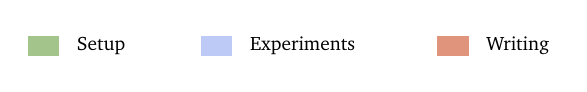
\begin{tikzpicture}
  \draw[fill=OliveGreen!40, draw=none] (0,0) rectangle (0.4,0.25);
  \node[right] at (0.5,0.125) {\scriptsize Setup};
  \draw[fill=RoyalBlue!35, draw=none] (2.2,0) rectangle (2.6,0.25);
  \node[right] at (2.7,0.125) {\scriptsize Experiments};
  \draw[fill=BrickRed!40, draw=none] (5.2,0) rectangle (5.6,0.25);
  \node[right] at (5.7,0.125) {\scriptsize Writing};
\end{tikzpicture}


\caption{Proposed research timeline.}
\label{fig:research_timeline}

\end{figure}

The implementation phase includes integration of the text refinement model with the downstream text-to-image diffusion pipeline. During this stage, tooling for prompt generation, inference automation, and evaluation logging will also be developed. Dataset preparation includes construction of structured compositional prompts and organisation of evaluation benchmarks such as T2I-CompBench++.

Experimental evaluation is expected to begin during July and August, focusing initially on baseline comparisons between raw prompting and refined prompting. Subsequent experiments investigate classifier-free guidance sensitivity and preservation of compositional structure under increasingly complex prompts. Quantitative and qualitative analyses will then be consolidated before dissertation writing and revision.

\section{Expected Deliverables}

The primary deliverable of this research is a completed MSc dissertation investigating diffusion-based refinement of textual conditioning for improved compositional generation in text-to-image diffusion models.

Additional research outputs include:

\begin{itemize}
    \item An implementation of the proposed conditioning refinement pipeline integrating diffusion-based text refinement with a pretrained text-to-image diffusion model.
    
    \item Experimental benchmark results comparing raw and refined conditioning across multiple compositional evaluation settings.
    
    \item Evaluation tooling for analysing compositional consistency, classifier-free guidance sensitivity, and role-filler preservation.
    
    \item A curated set of structured compositional prompts and evaluation scenarios used throughout experimentation.
    
    \item Potential conference or workshop publication material derived from the experimental findings.
\end{itemize}

These deliverables contribute both practically and theoretically. Practically, the work provides a reusable framework for evaluating conditioning quality in diffusion systems without requiring retraining of large-scale image generation models. Theoretically, the study contributes toward understanding conditioning representations as a central bottleneck in compositional generation.

\section{Risks and Mitigation Strategies}

Several practical risks may affect execution of the proposed experiments.

\subsection{Computational Constraints}

Diffusion-based image generation remains computationally intensive, particularly when evaluating multiple classifier-free guidance scales across large prompt sets. Long inference times may significantly slow experimentation.

To mitigate this risk, experiments will initially be conducted using reduced benchmark subsets and controlled sampling settings before scaling to larger evaluations. Generation will also be automated to allow asynchronous experiment execution and logging.

\subsection{Tooling and Integration Complexity}

Integrating diffusion-based text refinement models with downstream image generation pipelines may introduce implementation challenges, particularly regarding prompt formatting, token limits, and inference compatibility.

This risk will be mitigated through incremental development and validation of each pipeline component independently prior to full integration. Existing open-source diffusion frameworks and pretrained implementations will be used wherever possible to reduce engineering overhead.

\subsection{Evaluation Reliability}

Compositionality remains difficult to evaluate perfectly using automated metrics alone. Certain compositional failures may not be fully captured by benchmark scores.

To address this limitation, quantitative evaluation will be supplemented with structured qualitative analysis and visual inspection protocols. Scene graph consistency checks and VLM-based evaluation will also be used to strengthen reliability across evaluation settings.

\subsection{Resource Availability}

Availability of GPU compute resources may affect experimentation timelines and the scale of evaluations that can be performed.

Mitigation strategies include prioritising inference-only experimentation, using pretrained models rather than large-scale training, and conducting experiments using computationally efficient latent diffusion architectures.

\section{Research Limitations}

While the proposed methodology aims to provide controlled evaluation of conditioning refinement, several limitations remain.

First, the study focuses primarily on inference-time conditioning refinement rather than end-to-end retraining of diffusion models. As a result, the work cannot determine whether jointly optimising text refinement and image generation would produce further improvements.

Second, experiments will necessarily be conducted at smaller scales than those used in industrial text-to-image systems. Limitations in compute and dataset size may restrict the ability to fully evaluate emergent behaviours observed in large-scale generative models.

Third, evaluation benchmarks such as T2I-CompBench++ provide structured compositional tests but cannot exhaustively represent all forms of semantic reasoning required in real-world generation tasks. Consequently, improvements observed within benchmark settings may not generalise uniformly across all prompting scenarios.

Additionally, the proposed refinement model operates entirely within natural language space and therefore remains dependent on the representational capacity of the downstream text encoder. Even if prompts become semantically richer, some compositional information may still become partially entangled after projection into latent embedding space.

Finally, the study focuses specifically on compositional consistency and conditioning quality rather than photorealism or artistic generation quality. Improvements in compositionality may not necessarily translate into improvements across all perceptual dimensions of image generation.

Despite these limitations, the proposed work provides a focused and computationally feasible investigation into conditioning refinement as a mechanism for improving compositional reliability in diffusion-based generative systems.




\chapter{Conclusion}

This proposal presents a conditioning-centric approach to improving compositional image generation in text-to-image diffusion models. While recent advances in diffusion architectures have substantially improved image fidelity, compositional failures such as attribute misbinding, relational inconsistency, and sensitivity to prompt formulation remain persistent limitations.

This research argues that these failures arise not only from the generative model itself, but also from limitations in the conditioning representations used during sampling. In particular, textual prompts are compressed into latent embeddings in which explicit role-filler structure may become entangled or partially distorted before image generation begins. Under classifier-free guidance, such distortions may be further amplified during denoising.

To address this, the proposed work investigates whether diffusion-based refinement of textual prompts can improve the semantic structure of conditioning signals prior to encoding. By integrating GENIE into the conditioning pipeline without modifying the underlying image generation backbone, the study evaluates whether improved conditioning can reduce compositional errors and improve robustness to classifier-free guidance sensitivity.

The methodology combines compositional benchmarking, guidance sensitivity analysis, and role-filler evaluation to assess the downstream effects of conditioning refinement. Through this framework, the study seeks to contribute both empirical and theoretical insight into conditioning as a central bottleneck in diffusion-based generation.

If the proposed hypotheses are validated, this work will demonstrate that improving conditioning quality constitutes a viable and computationally efficient pathway toward more controllable and compositionally reliable generative models, without requiring architectural modification of existing diffusion systems.

\nocite{*}

\bibliography{references}\addcontentsline{toc}{chapter}{References}
\end{document}
